% Options for packages loaded elsewhere
\PassOptionsToPackage{unicode}{hyperref}
\PassOptionsToPackage{hyphens}{url}
\PassOptionsToPackage{dvipsnames,svgnames,x11names}{xcolor}
%
\documentclass[
  authoryear,
  preprint,
  3p,
  twocolumn]{elsarticle}

\usepackage{amsmath,amssymb}
\usepackage{iftex}
\ifPDFTeX
  \usepackage[T1]{fontenc}
  \usepackage[utf8]{inputenc}
  \usepackage{textcomp} % provide euro and other symbols
\else % if luatex or xetex
  \usepackage{unicode-math}
  \defaultfontfeatures{Scale=MatchLowercase}
  \defaultfontfeatures[\rmfamily]{Ligatures=TeX,Scale=1}
\fi
\usepackage{lmodern}
\ifPDFTeX\else  
    % xetex/luatex font selection
\fi
% Use upquote if available, for straight quotes in verbatim environments
\IfFileExists{upquote.sty}{\usepackage{upquote}}{}
\IfFileExists{microtype.sty}{% use microtype if available
  \usepackage[]{microtype}
  \UseMicrotypeSet[protrusion]{basicmath} % disable protrusion for tt fonts
}{}
\makeatletter
\@ifundefined{KOMAClassName}{% if non-KOMA class
  \IfFileExists{parskip.sty}{%
    \usepackage{parskip}
  }{% else
    \setlength{\parindent}{0pt}
    \setlength{\parskip}{6pt plus 2pt minus 1pt}}
}{% if KOMA class
  \KOMAoptions{parskip=half}}
\makeatother
\usepackage{xcolor}
\setlength{\emergencystretch}{3em} % prevent overfull lines
\setcounter{secnumdepth}{5}
% Make \paragraph and \subparagraph free-standing
\ifx\paragraph\undefined\else
  \let\oldparagraph\paragraph
  \renewcommand{\paragraph}[1]{\oldparagraph{#1}\mbox{}}
\fi
\ifx\subparagraph\undefined\else
  \let\oldsubparagraph\subparagraph
  \renewcommand{\subparagraph}[1]{\oldsubparagraph{#1}\mbox{}}
\fi

\usepackage{color}
\usepackage{fancyvrb}
\newcommand{\VerbBar}{|}
\newcommand{\VERB}{\Verb[commandchars=\\\{\}]}
\DefineVerbatimEnvironment{Highlighting}{Verbatim}{commandchars=\\\{\}}
% Add ',fontsize=\small' for more characters per line
\usepackage{framed}
\definecolor{shadecolor}{RGB}{241,243,245}
\newenvironment{Shaded}{\begin{snugshade}}{\end{snugshade}}
\newcommand{\AlertTok}[1]{\textcolor[rgb]{0.68,0.00,0.00}{#1}}
\newcommand{\AnnotationTok}[1]{\textcolor[rgb]{0.37,0.37,0.37}{#1}}
\newcommand{\AttributeTok}[1]{\textcolor[rgb]{0.40,0.45,0.13}{#1}}
\newcommand{\BaseNTok}[1]{\textcolor[rgb]{0.68,0.00,0.00}{#1}}
\newcommand{\BuiltInTok}[1]{\textcolor[rgb]{0.00,0.23,0.31}{#1}}
\newcommand{\CharTok}[1]{\textcolor[rgb]{0.13,0.47,0.30}{#1}}
\newcommand{\CommentTok}[1]{\textcolor[rgb]{0.37,0.37,0.37}{#1}}
\newcommand{\CommentVarTok}[1]{\textcolor[rgb]{0.37,0.37,0.37}{\textit{#1}}}
\newcommand{\ConstantTok}[1]{\textcolor[rgb]{0.56,0.35,0.01}{#1}}
\newcommand{\ControlFlowTok}[1]{\textcolor[rgb]{0.00,0.23,0.31}{#1}}
\newcommand{\DataTypeTok}[1]{\textcolor[rgb]{0.68,0.00,0.00}{#1}}
\newcommand{\DecValTok}[1]{\textcolor[rgb]{0.68,0.00,0.00}{#1}}
\newcommand{\DocumentationTok}[1]{\textcolor[rgb]{0.37,0.37,0.37}{\textit{#1}}}
\newcommand{\ErrorTok}[1]{\textcolor[rgb]{0.68,0.00,0.00}{#1}}
\newcommand{\ExtensionTok}[1]{\textcolor[rgb]{0.00,0.23,0.31}{#1}}
\newcommand{\FloatTok}[1]{\textcolor[rgb]{0.68,0.00,0.00}{#1}}
\newcommand{\FunctionTok}[1]{\textcolor[rgb]{0.28,0.35,0.67}{#1}}
\newcommand{\ImportTok}[1]{\textcolor[rgb]{0.00,0.46,0.62}{#1}}
\newcommand{\InformationTok}[1]{\textcolor[rgb]{0.37,0.37,0.37}{#1}}
\newcommand{\KeywordTok}[1]{\textcolor[rgb]{0.00,0.23,0.31}{#1}}
\newcommand{\NormalTok}[1]{\textcolor[rgb]{0.00,0.23,0.31}{#1}}
\newcommand{\OperatorTok}[1]{\textcolor[rgb]{0.37,0.37,0.37}{#1}}
\newcommand{\OtherTok}[1]{\textcolor[rgb]{0.00,0.23,0.31}{#1}}
\newcommand{\PreprocessorTok}[1]{\textcolor[rgb]{0.68,0.00,0.00}{#1}}
\newcommand{\RegionMarkerTok}[1]{\textcolor[rgb]{0.00,0.23,0.31}{#1}}
\newcommand{\SpecialCharTok}[1]{\textcolor[rgb]{0.37,0.37,0.37}{#1}}
\newcommand{\SpecialStringTok}[1]{\textcolor[rgb]{0.13,0.47,0.30}{#1}}
\newcommand{\StringTok}[1]{\textcolor[rgb]{0.13,0.47,0.30}{#1}}
\newcommand{\VariableTok}[1]{\textcolor[rgb]{0.07,0.07,0.07}{#1}}
\newcommand{\VerbatimStringTok}[1]{\textcolor[rgb]{0.13,0.47,0.30}{#1}}
\newcommand{\WarningTok}[1]{\textcolor[rgb]{0.37,0.37,0.37}{\textit{#1}}}

\providecommand{\tightlist}{%
  \setlength{\itemsep}{0pt}\setlength{\parskip}{0pt}}\usepackage{longtable,booktabs,array}
\usepackage{calc} % for calculating minipage widths
% Correct order of tables after \paragraph or \subparagraph
\usepackage{etoolbox}
\makeatletter
\patchcmd\longtable{\par}{\if@noskipsec\mbox{}\fi\par}{}{}
\makeatother
% Allow footnotes in longtable head/foot
\IfFileExists{footnotehyper.sty}{\usepackage{footnotehyper}}{\usepackage{footnote}}
\makesavenoteenv{longtable}
\usepackage{graphicx}
\makeatletter
\def\maxwidth{\ifdim\Gin@nat@width>\linewidth\linewidth\else\Gin@nat@width\fi}
\def\maxheight{\ifdim\Gin@nat@height>\textheight\textheight\else\Gin@nat@height\fi}
\makeatother
% Scale images if necessary, so that they will not overflow the page
% margins by default, and it is still possible to overwrite the defaults
% using explicit options in \includegraphics[width, height, ...]{}
\setkeys{Gin}{width=\maxwidth,height=\maxheight,keepaspectratio}
% Set default figure placement to htbp
\makeatletter
\def\fps@figure{htbp}
\makeatother

\makeatletter
\makeatother
\makeatletter
\makeatother
\makeatletter
\@ifpackageloaded{caption}{}{\usepackage{caption}}
\AtBeginDocument{%
\ifdefined\contentsname
  \renewcommand*\contentsname{Table of contents}
\else
  \newcommand\contentsname{Table of contents}
\fi
\ifdefined\listfigurename
  \renewcommand*\listfigurename{List of Figures}
\else
  \newcommand\listfigurename{List of Figures}
\fi
\ifdefined\listtablename
  \renewcommand*\listtablename{List of Tables}
\else
  \newcommand\listtablename{List of Tables}
\fi
\ifdefined\figurename
  \renewcommand*\figurename{Figura}
\else
  \newcommand\figurename{Figura}
\fi
\ifdefined\tablename
  \renewcommand*\tablename{Table}
\else
  \newcommand\tablename{Table}
\fi
}
\@ifpackageloaded{float}{}{\usepackage{float}}
\floatstyle{ruled}
\@ifundefined{c@chapter}{\newfloat{codelisting}{h}{lop}}{\newfloat{codelisting}{h}{lop}[chapter]}
\floatname{codelisting}{Listing}
\newcommand*\listoflistings{\listof{codelisting}{List of Listings}}
\makeatother
\makeatletter
\@ifpackageloaded{caption}{}{\usepackage{caption}}
\@ifpackageloaded{subcaption}{}{\usepackage{subcaption}}
\makeatother
\makeatletter
\@ifpackageloaded{tcolorbox}{}{\usepackage[skins,breakable]{tcolorbox}}
\makeatother
\makeatletter
\@ifundefined{shadecolor}{\definecolor{shadecolor}{rgb}{.97, .97, .97}}
\makeatother
\makeatletter
\makeatother
\makeatletter
\makeatother
\usepackage{float}
\makeatletter
\let\oldlt\longtable
\let\endoldlt\endlongtable
\def\longtable{\@ifnextchar[\longtable@i \longtable@ii}
\def\longtable@i[#1]{\begin{figure}[H]
\onecolumn
\begin{minipage}{0.5\textwidth}
\oldlt[#1]
}
\def\longtable@ii{\begin{figure}[H]
\onecolumn
\begin{minipage}{0.5\textwidth}
\oldlt
}
\def\endlongtable{\endoldlt
\end{minipage}
\twocolumn
\end{figure}}
\makeatother
\journal{Journal of Sea Research}
\ifLuaTeX
  \usepackage{selnolig}  % disable illegal ligatures
\fi
\usepackage[]{natbib}
\bibliographystyle{elsarticle-harv}
\IfFileExists{bookmark.sty}{\usepackage{bookmark}}{\usepackage{hyperref}}
\IfFileExists{xurl.sty}{\usepackage{xurl}}{} % add URL line breaks if available
\urlstyle{same} % disable monospaced font for URLs
\hypersetup{
  pdftitle={Diferencias en la composición de sustrato entre Dzilam de Bravo y El Cuyo de la península de Yucatán},
  pdfauthor={Sebastián Medina; David Sánchez; Diego Muñoz},
  pdfkeywords={keyword1, keyword2},
  colorlinks=true,
  linkcolor={blue},
  filecolor={Maroon},
  citecolor={Blue},
  urlcolor={Blue},
  pdfcreator={LaTeX via pandoc}}

\setlength{\parindent}{6pt}
\begin{document}

\begin{frontmatter}
\title{Diferencias en la composición de sustrato entre Dzilam de Bravo y
El Cuyo de la península de Yucatán \\\large{A Short Subtitle} }
\author[1]{Sebastián Medina%
\corref{cor1}%
\fnref{fn1}}
 \ead{319529818@enesmerida.unam.mx} 
\author[1]{David Sánchez%
%
\fnref{fn2}}
 \ead{420049609@enesmerida.unam.mx} 
\author[1]{Diego Muñoz%
%
\fnref{fn3}}
 \ead{317137150@enesmerida.unam.mx} 

\affiliation[1]{organization={ENES UNAM unidad Mérida, Ecología de Campo
VI},addressline={Tablaje Catastral N°6998, Carretera Mérida-Tetiz Km.
4.5},city={Ucú},postcode={97357},postcodesep={}}

\cortext[cor1]{Corresponding author}
\fntext[fn1]{This is the first author footnote.}
\fntext[fn2]{Another author footnote, this is a very long footnote and
it should be a really long footnote. But this footnote is not yet
sufficiently long enough to make two lines of footnote text.}
\fntext[fn3]{true}
        
\begin{abstract}
This is the abstract. Lorem ipsum dolor sit amet, consectetur adipiscing
elit. Vestibulum augue turpis, dictum non malesuada a, volutpat eget
velit. Nam placerat turpis purus, eu tristique ex tincidunt et. Mauris
sed augue eget turpis ultrices tincidunt. Sed et mi in leo porta
egestas. Aliquam non laoreet velit. Nunc quis ex vitae eros aliquet
auctor nec ac libero. Duis laoreet sapien eu mi luctus, in bibendum leo
molestie. Sed hendrerit diam diam, ac dapibus nisl volutpat vitae.
Aliquam bibendum varius libero, eu efficitur justo rutrum at. Sed at
tempus elit.
\end{abstract}



\begin{highlights}
\item Frase 1\item Frase 2\item Frase 3
\end{highlights}


\begin{keyword}
    keyword1 \sep 
    keyword2
\end{keyword}
\end{frontmatter}
    \ifdefined\Shaded\renewenvironment{Shaded}{\begin{tcolorbox}[breakable, frame hidden, boxrule=0pt, interior hidden, borderline west={3pt}{0pt}{shadecolor}, enhanced, sharp corners]}{\end{tcolorbox}}\fi

\hypertarget{introducciuxf3n}{%
\section{Introducción}\label{introducciuxf3n}}

Las zonas costeras representan un foco de interés para la biodiversidad,
pues son la base de intercambio de materia biótica y abiótica entre los
ecosistemas terrestres y los marinos. Estás albergan una gran diversidad
de especies en los ecosistemas que la conforman, específicamente uno de
ellos son los pastos marinos. Los pastos marinos están constituidos
principalmente por una comunidad vegetal bentónica
\citep{herrera2019pastos} distribuidos a manera de parches
estratificados. La península de Yucatán determinada por su estructura
geológica, se caracteriza por tener una amplia distribución de pastos
marinos. Esto es explicado por la poca profundidad que tienen sus
costas, permitiendo niveles de irradiación óptimos en amplias regiones.
Además de la composición calcárea de su sustrato que también favorece la
fijación y colonización de las plantas
macrofitas\citep{sanchez2007analisis}. Facilitando el crecimiento de una
variada macroflora marina.

Los pastos marinos cumplen con diferentes servicios ecosistémicos como,
la captura de carbono, ser disipador de corrientes permitiendo la
estructuración de las costas, así como, reducir las tasas de erosión
costera \citep{herrera2019pastos} y también como proveedor de
microhabitats para una gran diversidad de organismos invertebrados
considerados cómo fauna bentónica. La fauna bentónica es toda aquella
que se encuentra en el fondo del agua, clasificada en diferentes
tamaños: microbentónica \textless0.063 mm, meiobentónica 0.063--1.0 mm,
macrobentónica \textgreater1.0 mm y megabentónica \textgreater{} 10.0 mm
\citep{tagliapietra2010benthic}. Organismos como oligoquetos,
poliquetos, molúscos, gasterópodos, bivalvos, crustáceos, son fauna que
cumplen con ciertas funciones dentro de sus ecosistema, unas cumplen con
el papel de ser organismos detritívoros, otros como filtradores de
materia orgánica, y también están ligados dentro de la cadena trófica
como alimento para especies de mayor
tamaño\citep{tagliapietra2010benthic}.

Por consiguiente, estudiar la composición de las zonas costeras es una
tarea importante a realizar, ya que, de esta manera podríamos inferir en
la calidad de sustrato marino que se tiene y de la funciones ecológicas
que pudiera proveer. Teniendo una mayor referencia del estado de
conservación del sitio motivando a la caracterización y comparación de
dos zonas costeras de la península de Yucatán.

El propósito de este trabajo es caracterizar la composición del sustrato
submareal de Dzilam de Bravo y El Cuyo a 20, 40 y 60 metros de
la~línea~de~costa con el objetivo de comparar ambos sitios utilizando
una metodología AGRRA.

\hypertarget{metodologuxeda}{%
\section{Metodología}\label{metodologuxeda}}

\hypertarget{uxe1rea-de-estudio}{%
\subsection{\texorpdfstring{\emph{Área de
estudio}}{Área de estudio}}\label{uxe1rea-de-estudio}}

En este estudio contemplamos a Dzilam de Bravo y El Cuyo. El primero,
situado en el norte de Yucatán entre los paralelos 21°19' y 21°32' N y
los meridianos 88°35' y 88°58', limita al norte con el Golfo de México y
está influenciado en su circulación oceánica por los vientos y~ las
corrientes provenientes del canal de Yucatán, principalmente~
\citep{1834/36164}. Además, presenta una diversidad de fondos en la que
se encuentran fondos arenosos, arenosos con conchuela, duros de lajas y
piedras \citep{1834/36164}. Por su parte, El Cuyo se sitúa\ldots{}

\hypertarget{descripciuxf3n-de-muxe9todos-de-campo}{%
\subsection{\texorpdfstring{\emph{Descripción de métodos de
campo}}{Descripción de métodos de campo}}\label{descripciuxf3n-de-muxe9todos-de-campo}}

Empleando una versión modificada del protocolo AGRRA 2016-09-22 (Lang,
2016) para sustratos distintos a corales, demarcamos tres líneas de
muestreo paralelas a la playa que estuvieron separadas por 20 m entre
ellas a partir de la línea de costa. Cada línea de muestreo contuvo tres
transectos de 10 m separados por una distancia de 20 m entre ellos; cada
transecto fue marcado cada 10 cm a través de una soga. Para la
caracterización del sustrato, ocupamos una cámara Go Pro versión x para
grabar un video por transecto desde el inicio hasta el final de la soga
en el que se pudieran apreciar las marcas. Posteriormente, tomando en
cuenta lo que yaciera por debajo de cada marca, identificamos el
sustrato, o bien, las especies asociadas al mismo. Por otro lado, para
la caracterización del macrobentos sumareal, ocupamos un cuadrante de 25
x 25 cm que colocamos en los metros 1, 3, 5, 7 y 9 de cada transecto.
Dentro de cada uno de estos, despeluzamos gentilmente el sustrato en
búsqueda de animales bentónicos y registramos tal acción en un video de
30 segundos como mínimo.

\hypertarget{procesamiento-de-datos}{%
\subsection{\texorpdfstring{\emph{Procesamiento de
datos}}{Procesamiento de datos}}\label{procesamiento-de-datos}}

Los datos fueron procesados en RStudio versión 4.3.1. Las frecuencias de
presencia de cada tipo de sustrato por localidad fueron estandarizados
obteniendo su raíz cuarta. Posteriormente se generó una matriz de
disimilitud de Bray-Curtis con el paquete vegan (Oksanen et al., 2015).

\hypertarget{resultados}{%
\section{Resultados}\label{resultados}}

\hypertarget{discusiuxf3n}{%
\section{Discusión}\label{discusiuxf3n}}

\hypertarget{equations}{%
\section{Equations}\label{equations}}

Here is an equation: \[ 
  f_{X}(x) = \left(\frac{\alpha}{\beta}\right)
  \left(\frac{x}{\beta}\right)^{\alpha-1}
  e^{-\left(\frac{x}{\beta}\right)^{\alpha}}; 
  \alpha,\beta,x > 0 .
\]

Inline equations work as well: \(\sum_{i = 2}^\infty\{\alpha_i^\beta\}\)

\hypertarget{figures-and-tables}{%
\section{Figures and tables}\label{figures-and-tables}}

Fig.~\ref{fig-meaningless} is generated using an R chunk.

\begin{figure}

{\centering 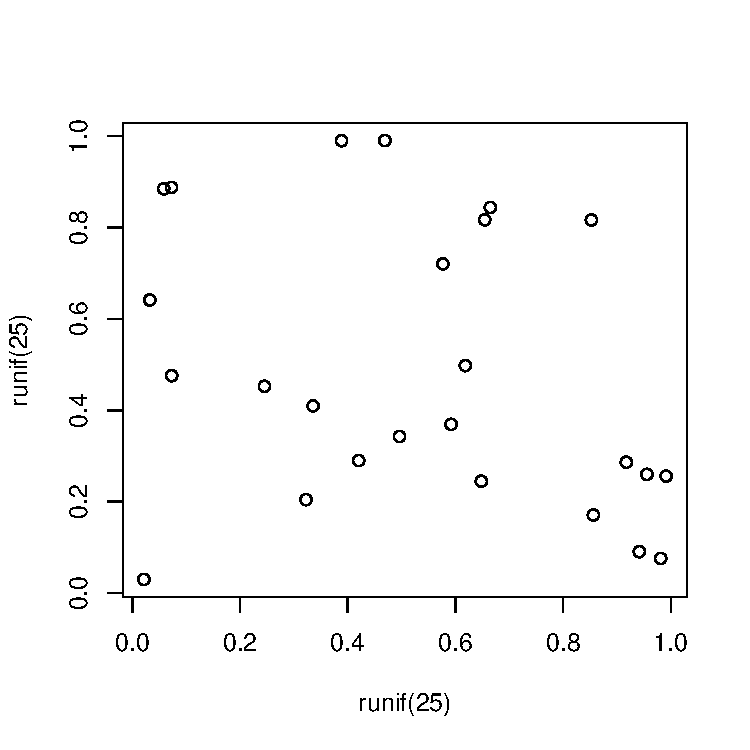
\includegraphics[width=0.5\textwidth,height=\textheight]{Reporte_Campo_files/figure-pdf/fig-meaningless-1.pdf}

}

\caption{\label{fig-meaningless}A meaningless scatterplot}

\end{figure}

\hypertarget{tables-coming-from-r}{%
\section{Tables coming from R}\label{tables-coming-from-r}}

Tables can also be generated using R chunks, as shown in
Table~\ref{tbl-simple} example.

\begin{Shaded}
\begin{Highlighting}[]
\NormalTok{knitr}\SpecialCharTok{::}\FunctionTok{kable}\NormalTok{(}\FunctionTok{head}\NormalTok{(mtcars)[,}\DecValTok{1}\SpecialCharTok{:}\DecValTok{4}\NormalTok{])}
\end{Highlighting}
\end{Shaded}

\hypertarget{tbl-simple}{}
\begin{longtable}[]{@{}lrrrr@{}}
\caption{\label{tbl-simple}Caption centered above table}\tabularnewline
\toprule\noalign{}
& mpg & cyl & disp & hp \\
\midrule\noalign{}
\endfirsthead
\toprule\noalign{}
& mpg & cyl & disp & hp \\
\midrule\noalign{}
\endhead
\bottomrule\noalign{}
\endlastfoot
Mazda RX4 & 21.0 & 6 & 160 & 110 \\
Mazda RX4 Wag & 21.0 & 6 & 160 & 110 \\
Datsun 710 & 22.8 & 4 & 108 & 93 \\
Hornet 4 Drive & 21.4 & 6 & 258 & 110 \\
Hornet Sportabout & 18.7 & 8 & 360 & 175 \\
Valiant & 18.1 & 6 & 225 & 105 \\
\end{longtable}


\renewcommand\refname{References}
  \bibliography{bibliography.bib}


\end{document}
